\section[IP Sec]{IP Sec: The Security Architecture for the Internet Protocol}
Die IP Security Architecture (IPSec) bietet Sicherheits-Features f�r einzelne Datenpakete. Urspr�nglich wurde diese Architektur zur Verwendung in IPv6 konstruiert. Die IPSec-Architektur wurde aber auch in die bisherige IP-Version (IPv4) aufgenommen. IPSec enth�lt alle Sicherheitsmechanismen, die zur Implementierung von VPNs n�tig sind. \newline
Die IPSec-Architektur besteht aus verschiedenen Protokollen, die IP-Header-Erweiterungen beschreiben, die Sicherheitsmechanismen bereitstellen. Die Sicherheitsfunktionen f�r die einzelnen Pakete werden durch zwei Protokolle bereitgestellt:
\paragraph{AH}
Der Authentication Header stellt Datenintegrit�t und Authentizit�t sicher.
\paragraph{ESP}
Das Encapsulating Security Payload-Protokoll sorgt f�r Privacy mit Hilfe von Verschl�sselungsmechanismen.
\newline
\newline
AH und ESP sind unabh�ngige Protokolle, sie separat oder miteinander kombiniert eingesetzt werden k�nnen.
\subsection[ESP]{The Encapsulation Security Payload}
Das ESP hat die Protokollnummer 50. Die Nutzdaten werden umfasst von einem ESP-Header und einem ESP-Trailer.
\begin{figure}[!htb]
	\centering
		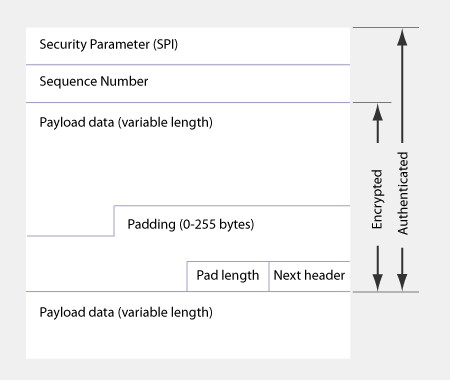
\includegraphics[width=0.50\textwidth]{figure_3_4.png}
\end{figure}
\newpage
\subsubsection{ESP header}
Der ESP-Header befindet sich zwischen IP- und TCP-/UDP-/...-Header. Er enth�lt einen sogenannten SPI (security parameter index), um die Sicherheits-Assoziation zu identifizieren, und eine Sequenznummer, die f�r jedes Datenpaket inkrementiert wird (Abwehr von Replay-Attacken).
\subsubsection{ESP trailer}
Der ESP-Trailer befindet sich hinter den Nutzdaten und ist, wie die Nutzdaten selbst, verschl�sselt. Der Trailer sorgt auch f�r das Padding (Auff�llen der Datenbl�cke), das n�tig ist, weil Verschl�sselungs-Algorithmen oft Datenbl�cke von einer bestimmten L�nge voraussetzen. Der Trailer enth�lt daher ein Feld, das die L�nge des Paddings in Bits enth�lt (pad length field). Ein weiteres Feld des ESP-Trailers enth�lt die Protokoll-Nummer des n�chsten Protokolls (z.B. IP oder ein ein n�chstes IPSec-Protokoll)
\subsection[AH]{The Authentication Header}
Das AH-Protokoll hat die Nummer 51. Es dient dazu, ein Datenpaket zu authentifizieren, so dass das IPSec-Peer des Empf�ngers sicher sein kann, von wo das erhaltene Paket stammt. Auch die Datenintegrit�t ist gew�hrleistet, d.h. die Empf�nger-Station kann �berpr�fen, dass kein Dritter das Paket w�hrend der �bertragung manipuliert hat. AH macht das durch das Berechnen von entsprechenden Authentifizierungs-Daten mit einer sicheren one-way Hash-Funktion. Da diese Berechnung mit Hilfe eines geheimen Schl�ssels geschieht. Ein Angreifer, der den geheimen Schl�ssel nicht kennt, ist nicht in der Lage, ein valides Datenpaket herauszufiltern oder zu authentifizieren. \newline Der AH-Header enth�lt ein Feld f�r den n�chsten Header und codiert die L�nge der Nutzdaten (n�tig, da die Authentifizierungsdaten variabel sind in ihrer L�nge). Wie der ESP-Header enth�lt auch der AH-Header einen SPI (Security Parameter Index) und eine Sequenznummer. Dahinter folgen dann die Authentifizierungsdaten (= der Wert der berechneten Hash-Funktion).
\begin{figure}[!htb]
	\centering
		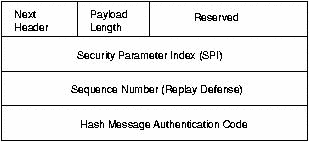
\includegraphics[width=0.50\textwidth]{ah_header.png}
\end{figure}
